\hypertarget{experiment-description}{%
\section{Experiment description}\label{experiment-description}}

\hypertarget{general-perspective}{%
\subsection{General perspective}\label{general-perspective}}

\begin{figure}[H]
\centering
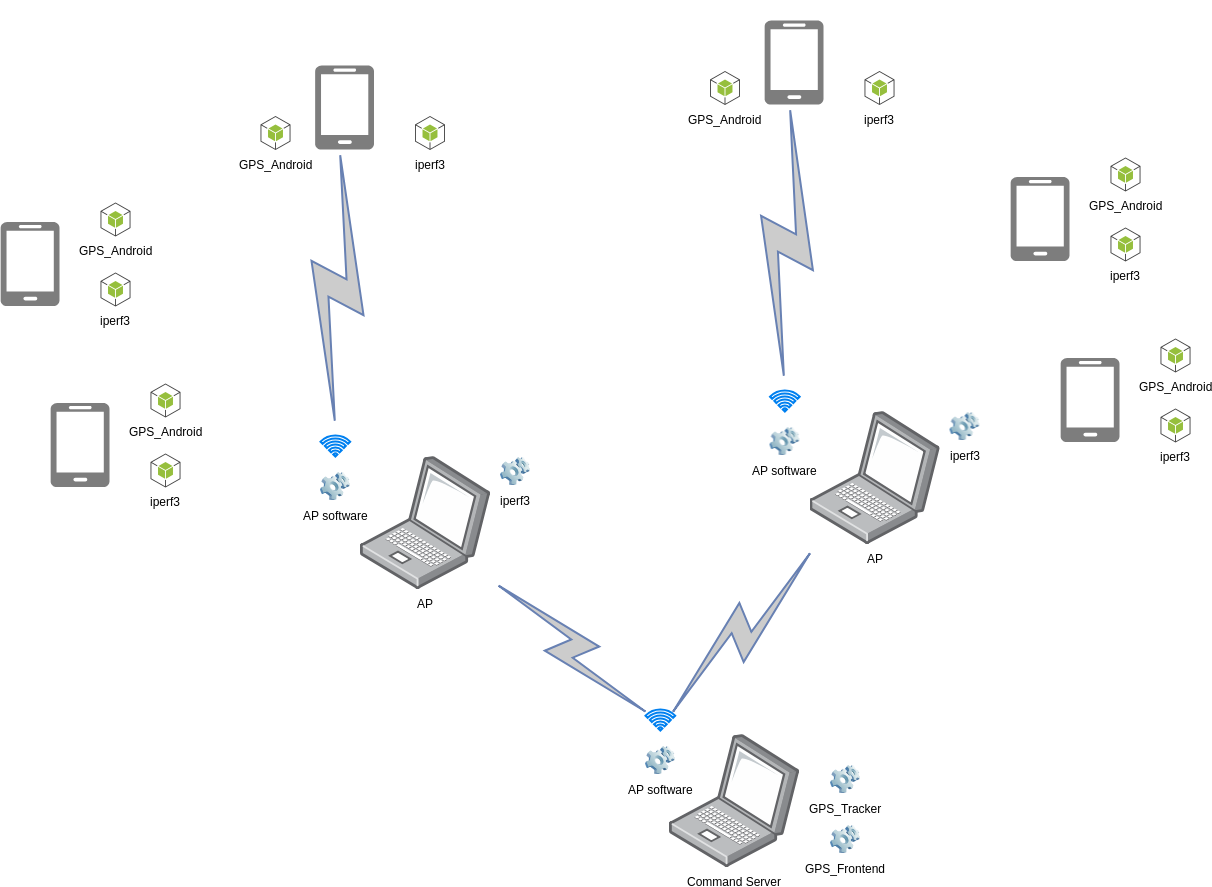
\includegraphics[width=\linewidth,keepaspectratio]{images/Deployment Diagram-Free-structure_scheme.png}
\caption{Main scenario of the experiment}
\label{fig:experiment-overall-layout}
\end{figure}

From the general system engineering perspective, the experiment is a set
of wireless-connected nodes (via Wi-Fi 802.11n (300 mbps)) which measures the receiving signal strength and measure the throughput of the link to upload and download.

All connections are wireless on each bearer:

\begin{itemize}
\tightlist
\item
  UE \textless{}-\textgreater{} AP.
\item
  AP \textless{}-\textgreater{} CnC.
\end{itemize}

There investigated one problem: the experimental network bandwidth
between UE and AP measurements with \texttt{iperf3} showed about
\textbf{30 MBit/s} speed rate. On the contrary, speed on the bearer UE \textless{}- AP -CnC\textgreater{} showed about \textbf{12-15 MBit/s} speed rate. There is markedly seen a drop in speed rate, probably, because of transmission on the radio channel two-times. The problem  is not in the Wi-Fi itself, but in the fact that radio (wireless) link is not as reliable, as a cord one, so the active bandwidth measurement part must be located as close to the APs as possible - in our case, the server-side \texttt{iperf3} is located in \acrshort{ap}s.

Each UE has two programs on board:

\begin{itemize}
\tightlist
\item
  \texttt{GPS\_Android} - special software designed to perform \acrshort{rss} and  link measurements linked to GPS coordinates.
\item
  \texttt{Magic\ iperf} - a network bandwidth measurement software.  Provides a user-friendly interface to client-side app \texttt{iperf}  on Android phones.
\end{itemize}

Each APs has two Wi-Fi adapters. Since we use laptops to run APs, they expected to have one already included, thus one external extra required for each AP. The internal Wi-Fi adapter connects to the CnC provided Wi-Fi network, the external Wi-Fi adapter creates the access point named
``\textbf{ap}'' for the UEs.

The CnC uses one external AP to create the access point named
``\textbf{cnc}''.

\hypertarget{deployment-diagram}{%
\subsection{Deployment Diagram}\label{deployment-diagram}}

\begin{longtable}[]{@{}ll@{}}
\caption{The main deployed components.}\tabularnewline
\toprule
\begin{minipage}[b]{0.16\columnwidth}\raggedright
Component\strut
\end{minipage} & \begin{minipage}[b]{0.78\columnwidth}\raggedright
Description\strut
\end{minipage}\tabularnewline
\midrule
\endfirsthead
\toprule
\begin{minipage}[b]{0.16\columnwidth}\raggedright
Component\strut
\end{minipage} & \begin{minipage}[b]{0.78\columnwidth}\raggedright
Description\strut
\end{minipage}\tabularnewline
\midrule
\endhead
\begin{minipage}[t]{0.16\columnwidth}\raggedright
Android smartphone group (UEs)\strut
\end{minipage} & \begin{minipage}[t]{0.78\columnwidth}\raggedright
A set of smartphones running Android OS (version 5.0+) with dedicated
Wi-Fi and installed software.\strut
\end{minipage}\tabularnewline
\begin{minipage}[t]{0.16\columnwidth}\raggedright
Access points (APs)\strut
\end{minipage} & \begin{minipage}[t]{0.78\columnwidth}\raggedright
The computers running a Wi-Fi AP software for the UEs connection. Pass
traffic through to CnC and take part in RSS and link quality
measurement.\strut
\end{minipage}\tabularnewline
\begin{minipage}[t]{0.16\columnwidth}\raggedright
Command Center (CnC)\strut
\end{minipage} & \begin{minipage}[t]{0.78\columnwidth}\raggedright
A computing node running the optimization software. Should be provided
with sufficient hardware resources.\strut
\end{minipage}\tabularnewline
\bottomrule
\end{longtable}

From the deployment view, we are using a complicated combination of
software and hardware.

We prefer to run AP and designed software separately in a virtual
machine. That helps to automate development, testing, and maintenance
routines.

\begin{figure}[H]
\centering
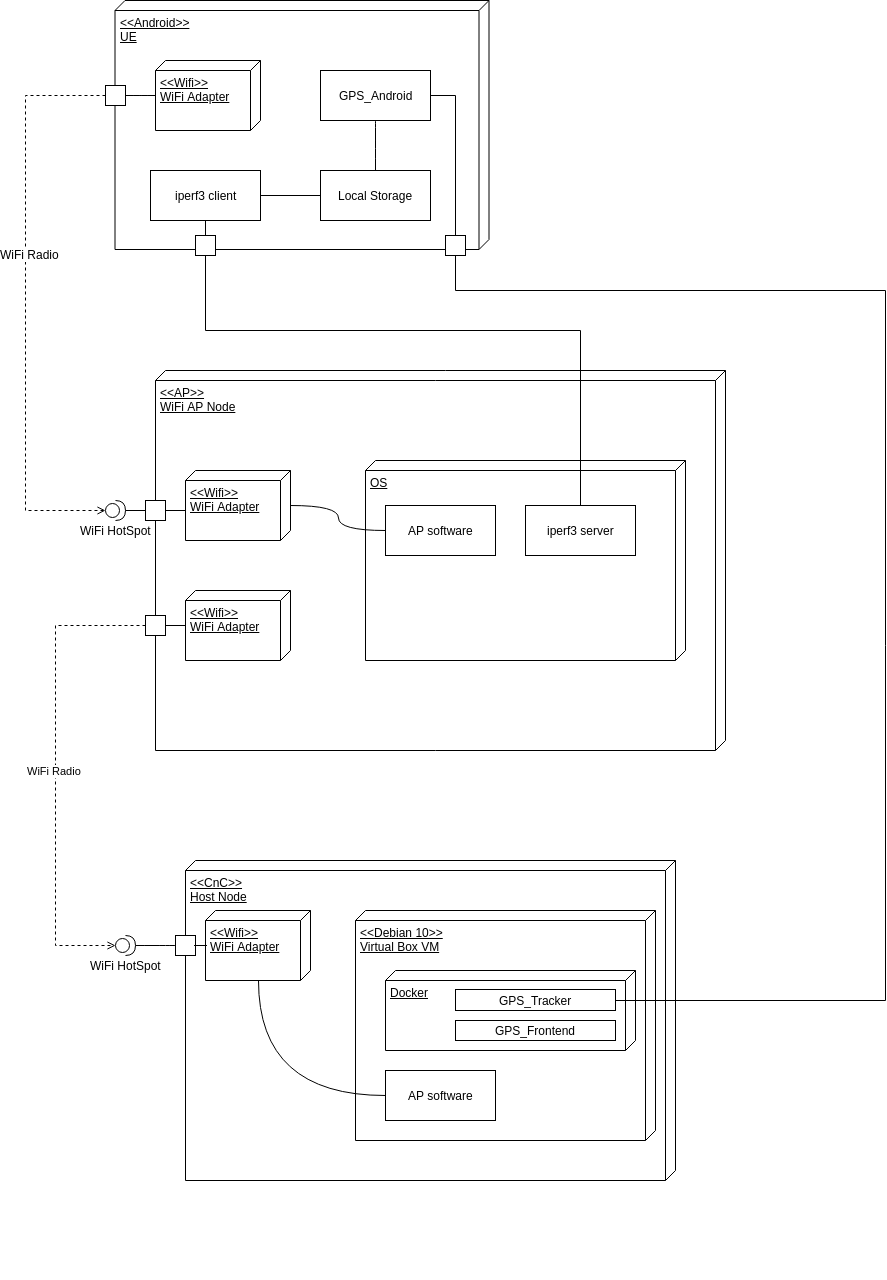
\includegraphics[width=\linewidth, keepaspectratio]{images/Deployment Diagram-Deployment_Diagram.png}
\caption{Deployment Diagram}
\label{fig:deployment-diagram}
\end{figure}

\hypertarget{command-center-deployment-cnc}{%
\subsubsection{Command center deployment
(CnC)}\label{command-center-deployment-cnc}}

The CnC software runs on Debian OS in VirtualBox virtual machine.
\texttt{GPS\_Tracker} and \texttt{GPS\_Frontend} are designed to run in
Docker containers. For the experiment, the virtual machine has \textbf{docker}
and \textbf{docker-compose} installed to run these containers. It possible to have performance decrease because of running in containers, however more powerful hardware resources compensates those possible consequences of additional run-time level.

The AP software consists of two packages:

\begin{itemize}
\tightlist
\item
  \texttt{hostapd} - software to manage and run Wi-Fi access points.
\item
  \texttt{dnsmasq} - DNS/DHCP server, to provide an IP address, routing
  and DNS information via DHCP protocol.
\end{itemize}

The AP software starts in the virtual machine, which can access the physical Wi-Fi adapter using the hardware pass-through function from the host machine.

For easy-to-run configuration and deployment of the CnC, there are
provided an \textbf{Ansible} script.

\hypertarget{access-points-deployment-aps}{%
\subsubsection{Access Points deployment
(APs)}\label{access-points-deployment-aps}}

Unlike CnC, physical nodes run the AP software and server-side
\texttt{iperf3} app.

\hypertarget{network-diagram}{%
\subsection{Network Diagram}\label{network-diagram}}

The APs subnet has identical settings. These
\texttt{Wi-Fi\ HotSpot\ Network} has an internal DHCP server to provide
dynamic addresses for connected UEs. To prevent the network IP addresses
collisions and simplify routing, the APs perform masquerading
(SNAT/DNAT) on the output interface (the internal interface used to
connect to CnC). On the one side, it cannot access the UEs directly from
CnC, but the UEs will always reach CnC as long as DHCP sets the default
gateway IP address.

In \texttt{Wi-Fi\ CnC\ Network} installed another DHCP server. It used
to reply to connecting APs with dynamic addresses. Because the subnet
used in this network is different from the internal Wi-Fi adapter's
network in the APs, there is no network collision.

Finally, the UEs can access the static CnC address \texttt{192.168.20.1}
as well as its local AP's gateway address \texttt{192.168.10.1}.


\begin{figure}[H]
	\centering
	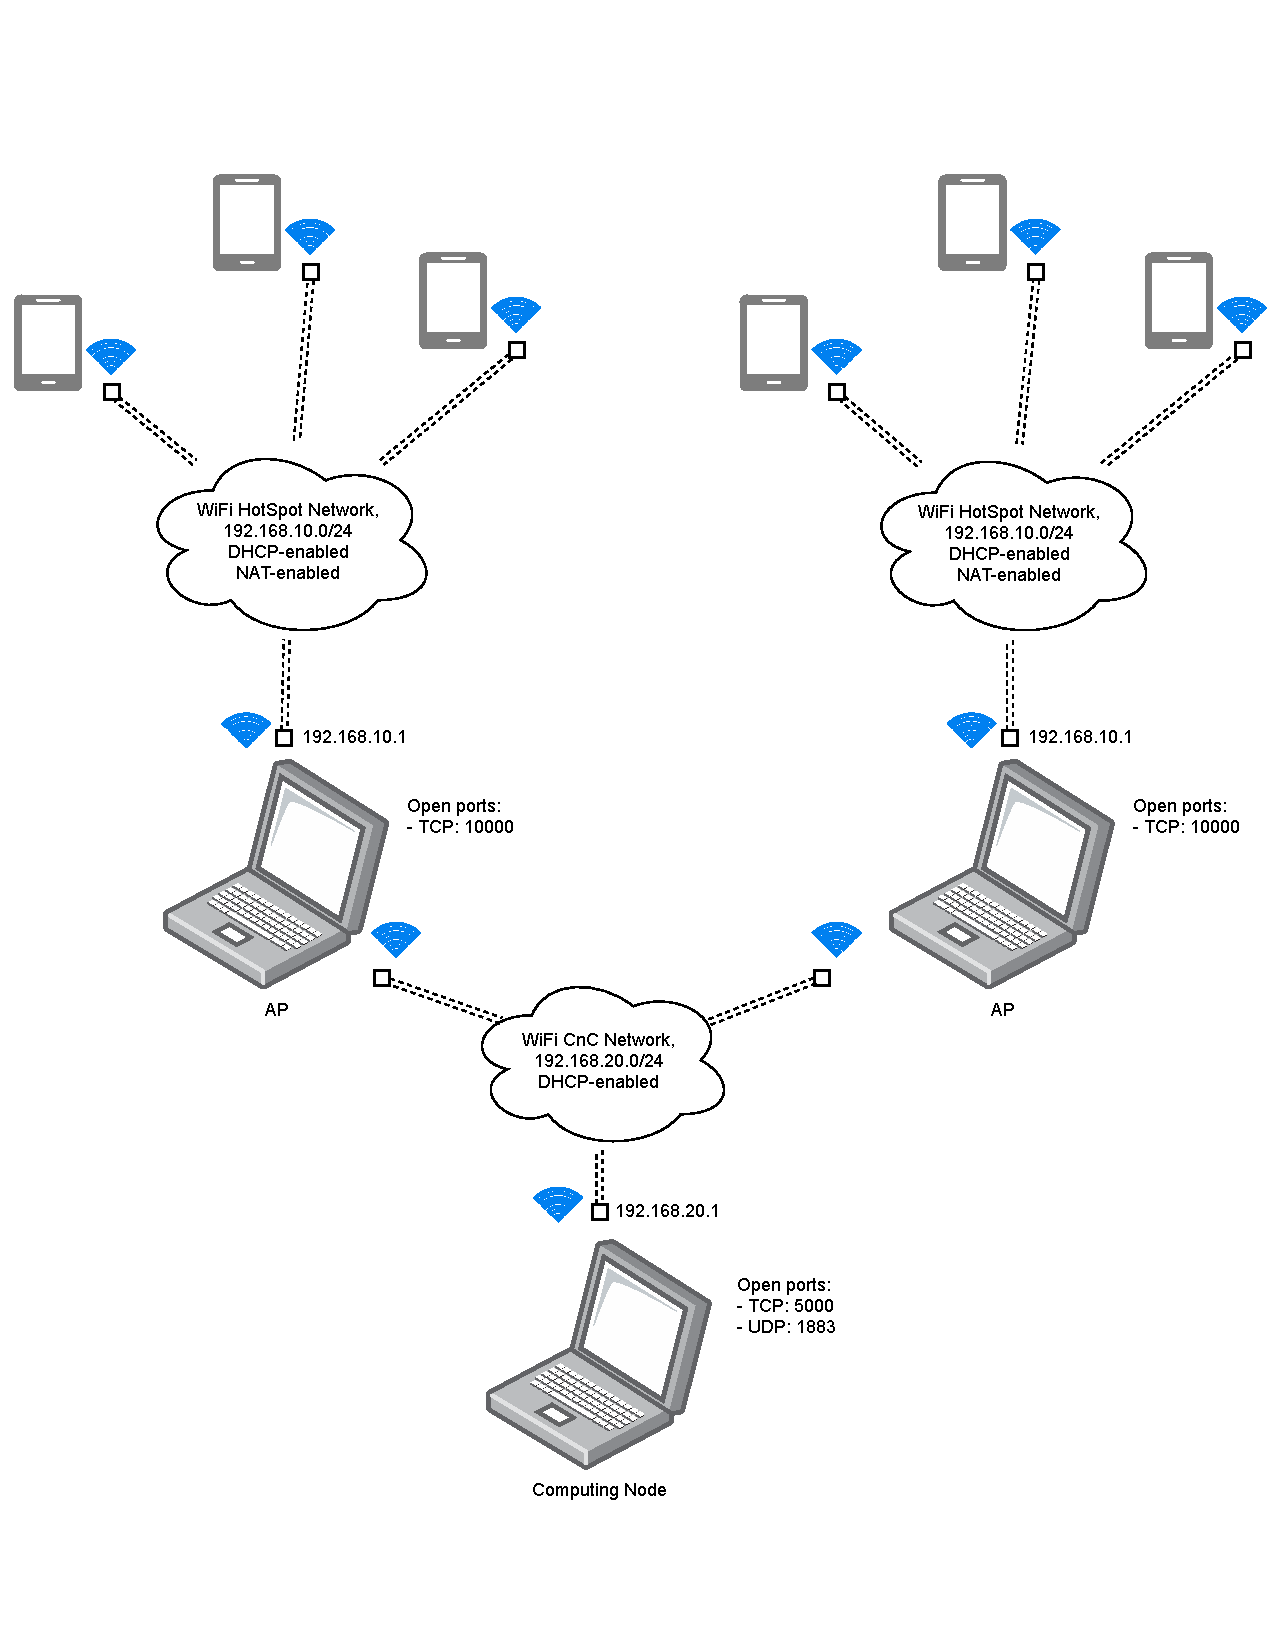
\includegraphics[width=0.3\linewidth, keepaspectratio]{images/Deployment Diagram-Network_Diagram.pdf}
\caption{Network Diagram}
\label{fig:network-diagram}
\end{figure}

\hypertarget{experiment-steps}{%
\subsection{Experiment Steps}\label{experiment-steps}}

The following steps will be executed for each described experimental
case:

\begin{longtable}[]{@{}lll@{}}
\caption{Steps for one experimental case.}\tabularnewline
\toprule
\begin{minipage}[b]{0.01\columnwidth}\raggedright
No\strut
\end{minipage} & \begin{minipage}[b]{0.35\columnwidth}\raggedright
Step\strut
\end{minipage} & \begin{minipage}[b]{0.55\columnwidth}\raggedright
Description\strut
\end{minipage}\tabularnewline
\midrule
\endfirsthead
\toprule
\begin{minipage}[b]{0.01\columnwidth}\raggedright
No\strut
\end{minipage} & \begin{minipage}[b]{0.35\columnwidth}\raggedright
Step\strut
\end{minipage} & \begin{minipage}[b]{0.55\columnwidth}\raggedright
Description\strut
\end{minipage}\tabularnewline
\midrule
\endhead
\begin{minipage}[t]{0.01\columnwidth}\raggedright
1\strut
\end{minipage} & \begin{minipage}[t]{0.35\columnwidth}\raggedright
Initialize network connectivity between APs and CnCs\strut
\end{minipage} & \begin{minipage}[t]{0.55\columnwidth}\raggedright
Ensure that these nodes are available in the network by the ICMP
protocol\strut
\end{minipage}\tabularnewline
\begin{minipage}[t]{0.01\columnwidth}\raggedright
2\strut
\end{minipage} & \begin{minipage}[t]{0.35\columnwidth}\raggedright
Run the software for the experiment\strut
\end{minipage} & \begin{minipage}[t]{0.55\columnwidth}\raggedright
Startup GPS\_Tracker, GPS\_Frontend\strut
\end{minipage}\tabularnewline
\begin{minipage}[t]{0.01\columnwidth}\raggedright
3\strut
\end{minipage} & \begin{minipage}[t]{0.35\columnwidth}\raggedright
Place the APs and UEs according to an experiment case\strut
\end{minipage} & \begin{minipage}[t]{0.55\columnwidth}\raggedright
There are specific predefined positions for each element on the
experiment area.\strut
\end{minipage}\tabularnewline
\begin{minipage}[t]{0.01\columnwidth}\raggedright
4\strut
\end{minipage} & \begin{minipage}[t]{0.35\columnwidth}\raggedright
Measure RSS, Link quality for the initial layout\strut
\end{minipage} & \begin{minipage}[t]{0.55\columnwidth}\raggedright
Measurements are done via GPS\_Android that sends the result to
GPS\_Tracker\strut
\end{minipage}\tabularnewline
\begin{minipage}[t]{0.01\columnwidth}\raggedright
5\strut
\end{minipage} & \begin{minipage}[t]{0.35\columnwidth}\raggedright
Run the APs location optimization for each algorithm in
GPS\_Tracker\strut
\end{minipage} & \begin{minipage}[t]{0.55\columnwidth}\raggedright
Each optimization algorithm can produce different probable positions for
the same UE positions and measurements.\strut
\end{minipage}\tabularnewline
\begin{minipage}[t]{0.01\columnwidth}\raggedright
6\strut
\end{minipage} & \begin{minipage}[t]{0.35\columnwidth}\raggedright
Move the APs to the optimized positions\strut
\end{minipage} & \begin{minipage}[t]{0.55\columnwidth}\raggedright
It is expected that new positions for APs would increase our network
efficiency.\strut
\end{minipage}\tabularnewline
\begin{minipage}[t]{0.01\columnwidth}\raggedright
7\strut
\end{minipage} & \begin{minipage}[t]{0.35\columnwidth}\raggedright
Repeat RSS and Link quality measurements for the optimized APs
positions\strut
\end{minipage} & \begin{minipage}[t]{0.55\columnwidth}\raggedright
1-3 interactions for optimization per each case.\strut
\end{minipage}\tabularnewline
\bottomrule
\end{longtable}
